\documentclass[10pt,letterpaper]{article}

\usepackage{cogsci}
\usepackage{pslatex}
\usepackage{apacite}
\usepackage{graphicx}
\usepackage{natbib}

\title{Memory Driven Temporal Preparation: A Cognitive Model}
 
\author{{\large \bf Steven Bosch (s1861948)} \\
  Faculty of Mathematics and Natural Sciences}


\begin{document}
\maketitle

\begin{abstract}
Blabla

\textbf{Keywords:} 
temporal preparation; cue target interval timing; Hazard function; long term memory
\end{abstract}

\section{Introduction}
The human brain has many traits that we are hardly aware of during our everyday lives, even though these traits have a great impact on our experiences and actions. One such trait is the ability of cue target interval timing. Both consciously and unconsciously this ability is exercised in numerous situations, such as waiting for traffic lights, expecting a sound when something falls or simply expecting the second hand of a clock to move to the next second. What are the cognitive mechanisms behind this ability?

One theory encompasses the \textit{Hazard function}. This function describes that the conditional probability of the occurrence of a target event after the presentation of a cue increases over time given that the event has not yet occurred. While this function has been successfully used to predict interval timing behaviour \cite{Nobre, Vangkilde}, it does not provide an explanation as to the cognitive processes behind it. Moreover it does not take into account memory traces of preceding timing experiences. The past years research began on this basis \cite{Los1, Howard, Taatgen}. Los et al. (2014) developed what they called the \textit{multiple trace theory of temporal preparation} (MTP), in which every new trial causes a memory trace to be created, storing a temporal profile of that trial.This memory trace subsequently contributes to the preparation of subsequent trials. 

A recent experiment by Los et al. indicated that temporal preparation is indeed driven by memory \cite{Los2}. In the experiment different groups of participants were presented with different distributions of foreperiods between temporal cues and target stimuli. Three of these experiments showed a transfer effect of this manipulation in a test phase where all participants received the same uniform distribution, indicating memory influence. 

This paper discusses a model that tries to capture (some of) the cognitive processes behind the phenomenon that the experiment by Los et al. (2015) brought to light. Using a cognitive model might give us more insight into he workings of this particular cognitive process.

\section{Experiment}
\subsection{Method}
In Los et al.'s (2015) experiment sixty-four students were randomly assigned to one of two groups, each consisting of 32 participants. The participants were asked to sit behind a computer screen with their left index finger on the \textit{z} key and their right index finger on the \textit{m} key. Each trial started with the appearance of a black plus sign, \textit{S1}, in the middle of the screen. Subsequently after a given foreperiod of either 400, 800, 1200 or 1600 ms a second signal, \textit{S2}, appeared. Seeing the signal, the participants had to press either \textit{z}, when \textit{S2} appeared left, or \textit{m} when \textit{S2} appeared right. They were instructed to perform this action as fast as they could. After the response the screen turned black and after an interval of 1.5 seconds the next trial would start.

Every participant had to complete 5 blocks of 120 trials each. The distribution of trials within a block was either uniform (30 trials of each foreperiod), exponential (64, 32, 16 and 8 trials for foreperiods of 400, 800, 1200 and 1600 ms respectively) or anti-exponential (8, 16, 32 and 64 trials for foreperiods of 400, 800, 1200 and 1600 ms respectively) distribution. Table \ref{Table1} shows the foreperiod distributions of the blocks per group. For both of the groups block 1, 4 and 5 were uniform, whereas block 2 and 3 were either exponential or anti-exponential.

In the experiment the participants were informed every block about their mean response time (RT) and the percentage of correct responses of that block. Furthermore after block 3 they were informed of the distributions of the preceding and succeeding two blocks.

\begin{table}
	\centering
	\caption{Successive foreperiod distributions across blocks for group 1 and 2 (Uni \= uniform, Exp \= exponential, Anti-exp \= anti-exponential).}
	\begin{tabular}{c|c|c|c|c|c}
		Block & 1 & 2 & 3 & 4 & 5 \\
		\hline
		Group 1 & Uni & Exp & Exp & Uni & Uni \\
		Group2 & Uni & Anti-exp & Anti-exp & Uni & Uni
	\end{tabular}
	\label{Table1}
\end{table}

\subsection{Results}
Figure \ref{LosFigure} shows the results of Los et al.'s experiment. Los et al. themselves applied a mixed Analysis of Variance (ANOVA) on the data of each block, with group and foreperiod as factors. They report a strong main effect of foreperiod in all blocks, minimal $F (1, 62) = 58.63$ and $p < 0.001$. Furthermore they reported a significant main effect of group in block 2, $F (1, 62) = 13.81$, $p < 0.001$ and 3, $F(1, 62) = 13.95$, $p < 0.001$, but not in the other blocks. The interaction between group and foreperiod was not significant in block 1, $F(1, 62) < 1$, but it was in the other four blocks, with blocks 2 and 3 having minimal $F (1, 62) = 69.64$, $p < 0.001$, and blocks 4 and 5 having minimal $F (1, 62) = 13.12$ and $p \leq 0.001$.

Figure \ref{LosFigure} shows that for the first uniform distribution, when the participants do not have any prior experience with the experiment yet, their mean RT fore a foreperiod of 400 ms is around 360 ms. It decreases exponentially to around 320 ms for a foreperiod of 1600. In blocks 2 and 3 we see a clear difference between the exponential and anti-exponential distribution. The mean RT for the exponential group decreases greatly for shorter foreperiods, while the opposite happens for the anti-exponential group: the mean RT increases especially for the shorter foreperiods. In the final two blocks we can still see slight remnants of the preceding distributions, with slight differences between the two groups of participants (as discussed the interactino between group and foreperiod was significant in these blocks as well).

As discussed in the introduction, from these results it appears that the cognitive process of cue target interval timing involves more than just the hazard function. Indeed, otherwise there would have been no difference between the mean RTs of the different blocks. The results of this experiment clearly showed that the distribution of foreperiods does affect the anticipation of the second stimulus. When many short stimuli have appeared in the recent experiences of a participant, he will be more prone to react faster after a short foreperiod. Similarly when many long stimuli have appeared in his recent experiences, the response time is longer for all foreperiods, but especially for the shorter ones. This observation brings us to the cognitive model this study discusses.

\begin{figure}
	\centering
	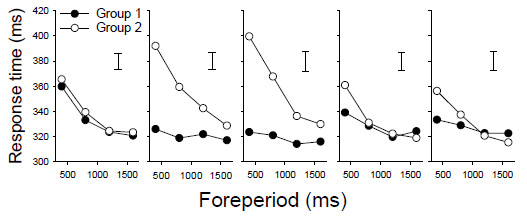
\includegraphics[width=\columnwidth]{Los1.png}
	\caption{Los et al.'s experiment results of mean response time as a function of group, block and foreperiod. Illustration from Los et al. (2015).}
	\label{LosFigure}
\end{figure}

\section{Model}
\subsection{Method}
The model consists of a timing and memory function, which were built upon functions that are proposed earlier in the literature, and two components specifically designed for the current timing task. 

The timing function is modelled by \citet{Taatgen1} as an Act-R module, the `temporal module'.\footnote{Act-R is a cognitive architecture, see http://act-r.psy.cmu.edu/.}. This module models the idea that people internally measure an interval in number of ticks, which are counted with increasingly long intervals. Furthermore the model uses a memory function that is proposed in \citet{Taatgen}, in which memories are stored as encounters of a specific chunk in the declarative memory. Subsequently the activation of every chunk their prior probabilities are calculated (the probability of retrieving the concerned memory).

For this specific cue target interval timing problem there were two more main components that needed to be modelled, in order for the model to produce the results generated in the experiment:
\begin{enumerate}
	\item A hazard function
	\item Memory influence on the temporal preparation
\end{enumerate}
Let us discuss each of these separately.

\paragraph{The hazard function}
The hazard function is necessary, because the first block in the experiment clearly showed that without memory of past cue target timing experiences, the mean response times decrease logarithmically as the foreperiod becomes longer, down to a certain threshold.\footnote{Note that this study only discusses the time intervals discussed in Los et al.'s paper. Different mechanisms might come into play for shorter or longer intervals.} The Hazard function can be applied here: the longer it takes before the second signal is shown, the higher the probability becomes that it will come at the next millisecond. 

The fact that the plots show some sort of negative logarithmic function might be the result of a number of things. First, there is a limit to how fast a human being can respond: he has to observe the signal first, after which this image has to be processed and recognized. Finally the procedural step has to be taken to press the (right) button. Since all of these processes take time, it is logical that there is an asymptote that the response times approach as the participants become more prepared. They can never be faster than a certain speed. Second, a participant cannot expect the experiment to last forever. This makes it logical that the first milliseconds its expectation increases (so its response time decreases) at a higher rate than at a later time. 

Finally, one last assumption is made in modelling the hazard function: there is also a maximum response time. No matter how ill-prepared a participant may be for the second signal, he will still respond within a certain amount of time, unless of course he is distracted in one way or another.

The implementation of the Hazard function used in the model is the following:
\begin{equation}
	R = R_b + maxDelay * e^{-\frac{ticks^d}{m}}
\end{equation}
Here $R$ is the response time, $R_b$ the base response, maxDelay the maximum number of milliseconds a response can take, ticks the number of ticks counted during the foreperiod, and $d$ and $m$ parameters that depend on memory (see the next paragraph). This study uses a base response of 320 ms and a maximum delay of 150 ms, meaning that all of the responses fall within 320 and 470 ms. The exponential factor in the function makes sure that a longer foreperiod is always responded to more quickly than a shorter one. It depends on $d$ and $m$ what the magnitude of this difference is.

\paragraph{Memory influence}
From the results of the Los et al. experiment it appears that memory has a direct influence on the preparation rate for the second signal. 

\begin{figure}
	\centering
	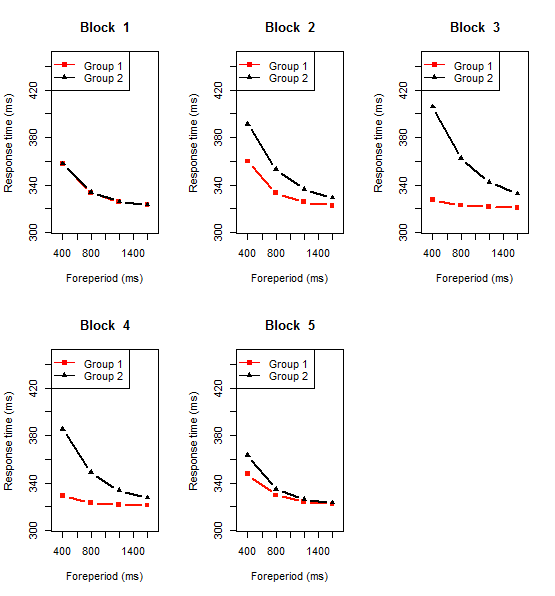
\includegraphics[width=\columnwidth]{5blocks2.png}
	\caption{Model results of mean response time as a function of group, block and foreperiod.}
	\label{5blocks}
\end{figure}

\section{Discussion}



\bibliographystyle{apacite}
\setlength{\bibleftmargin}{.125in}
\setlength{\bibindent}{-\bibleftmargin}
\bibliography{bibliography}

\end{document}
